\documentclass{article}

\usepackage{geometry}
\usepackage{graphicx}

\title{Exercise 2 -- Lab 1 Man in the Middle}
\author{Stewart Johnston\\
  {CIS 127 -- Intro to Information Security}\\
  {NCMC}\\
  {\texttt{johnstons1@student.ncmich.edu}}
}
\date{}

\begin{document}
\maketitle

\section{Listening to SSH over the wire}

In the lab, an ssh connection was made to an amazon aws server. When the client
and server initially connect, a sparse amount of information is sent, and can
be gleaned from the packets. As can be noted from the screenshots, the exact
version of SSH and its underlying version can be seen, per \ref{fig:ssh1}. The kind of key
encryption is discussed, but not the keys themselves. And... that's it. All
other information from that point on is cyphertext, and cannot be read unless
in possession of the encryption underneath it.

\begin{figure}[h]
	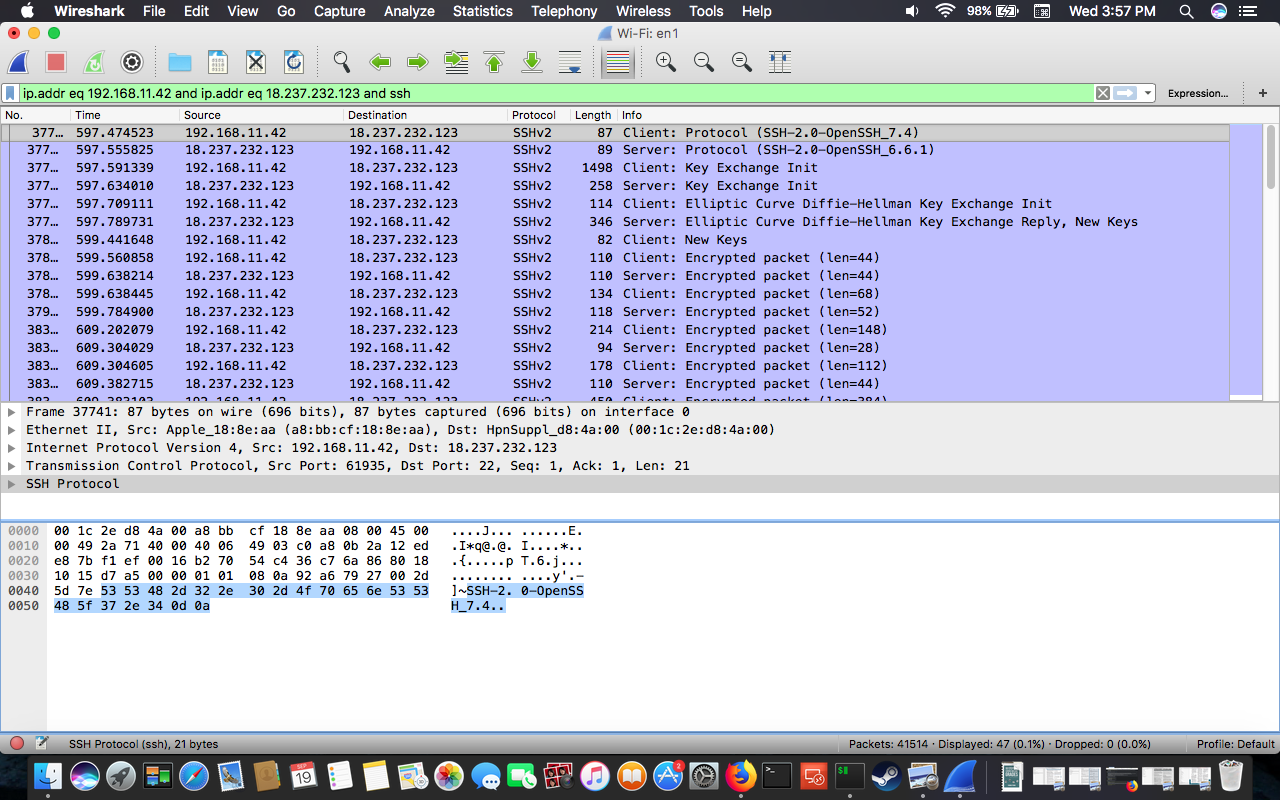
\includegraphics[width=\linewidth]{ssh1.png}
	\caption{Client information visible}
	\label{fig:ssh1}
\end{figure}
\begin{figure}[h]
	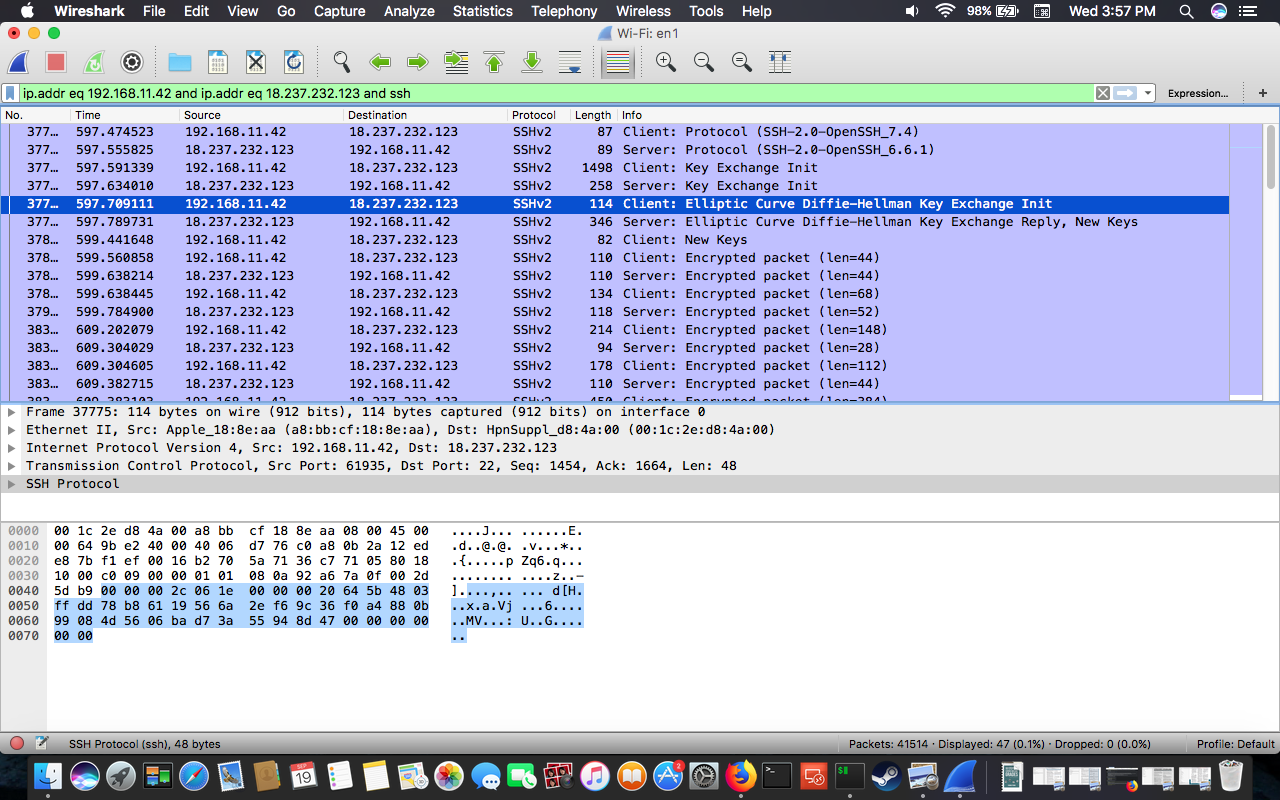
\includegraphics[width=\linewidth]{ssh2.png}
	\caption{}
	\label{}
\end{figure}
\begin{figure}[h]
	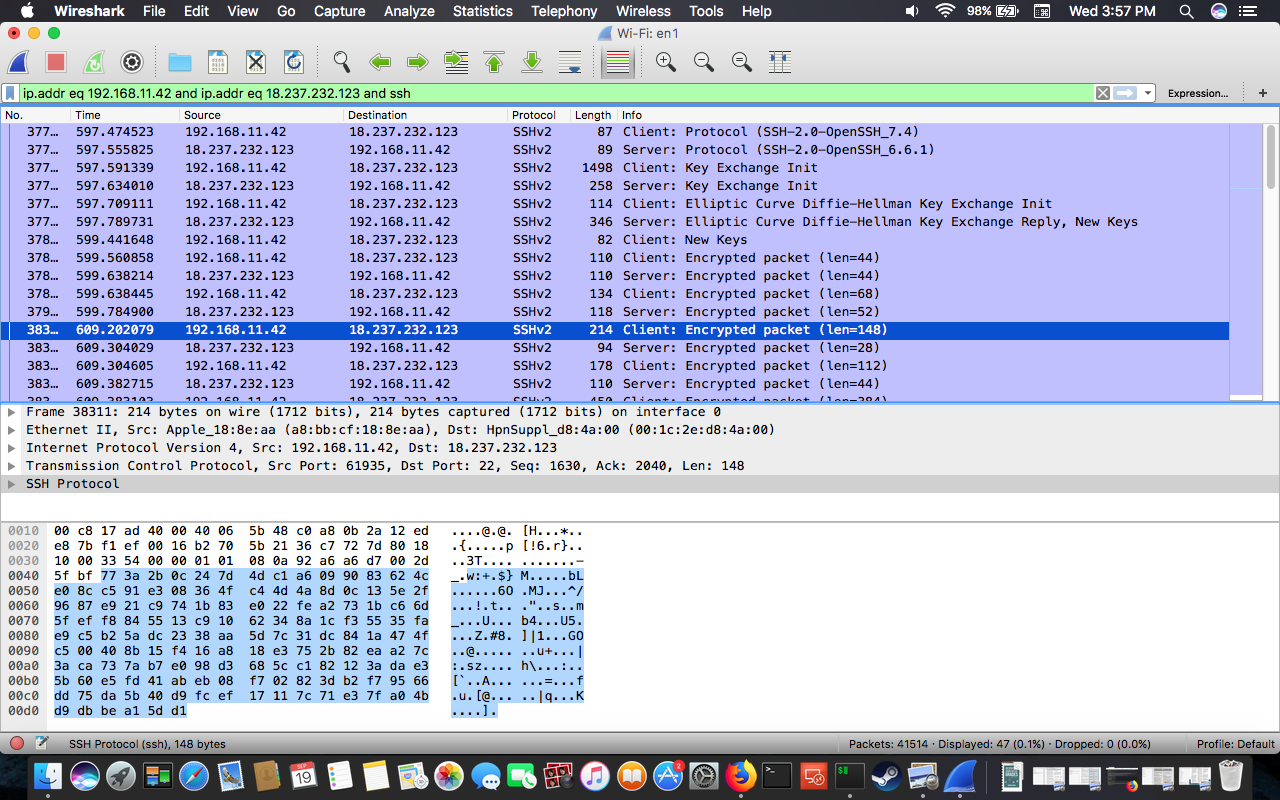
\includegraphics[width=\linewidth]{ssh3.png}
	\caption{}
	\label{}
\end{figure}

\section{Listening to Telnet over the wire}

Telnet was certainly not as secure, as every part of the transmission was in
cleartext. The exact kind of client could be seen per \ref{fig:telnet1}, as well as
the target user and password, as in \ref{fig:telnet3}. By extension, all details sent over the
connection, as with any other cleartext connection, could be grabbed off of the
wire or out of the air. Telnet is by no means a secure program to use for
connecting to a remote server.

\begin{figure}[h]
	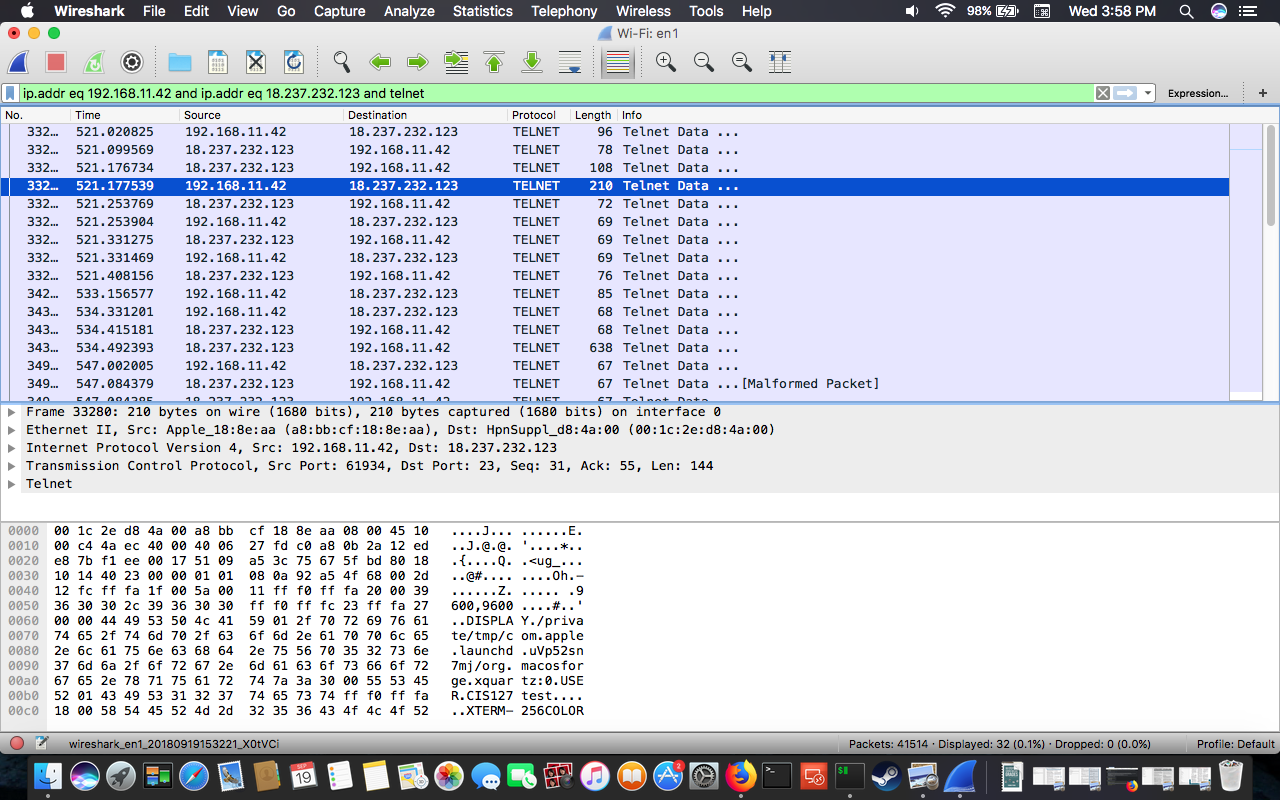
\includegraphics[width=\linewidth]{telnet1.png}
	\caption{Information in the clear! Not good.}
	\label{fig:telnet1}
\end{figure}
\begin{figure}[h]
	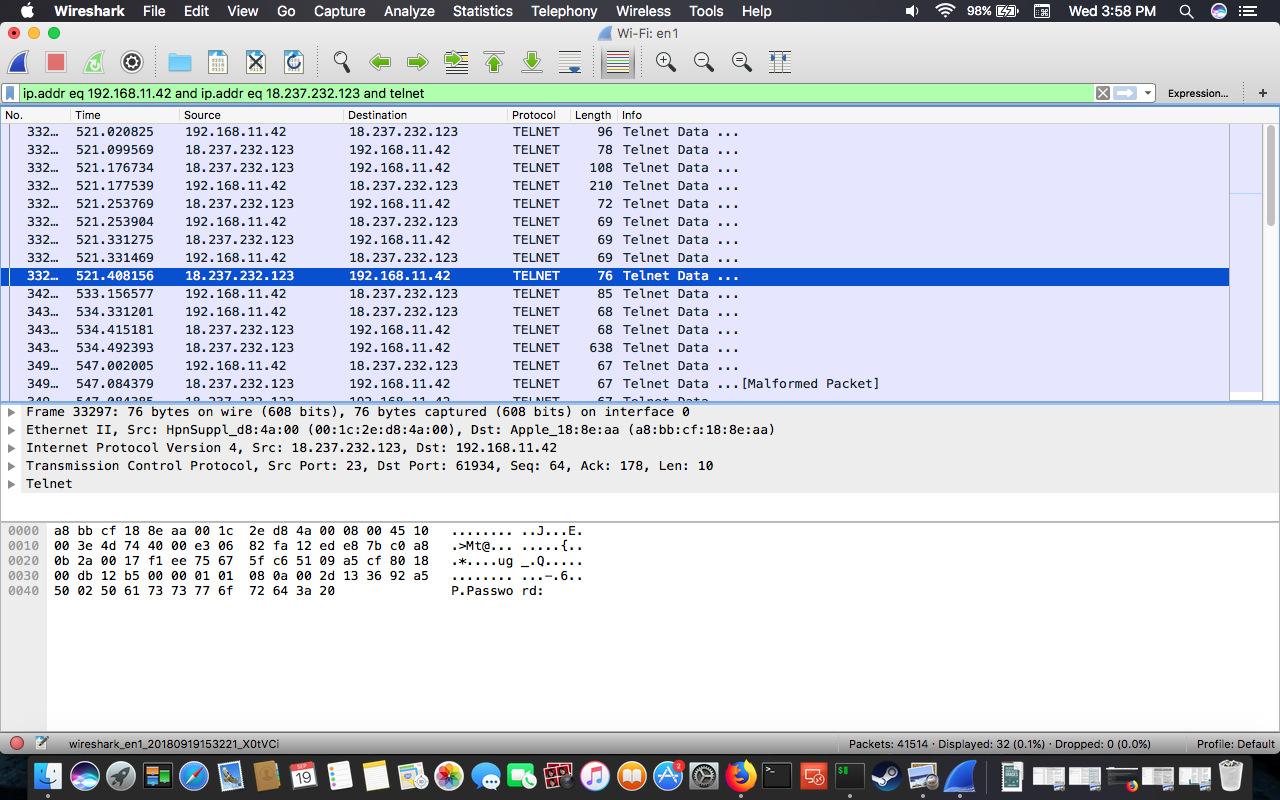
\includegraphics[width=\linewidth]{telnet2.png}
	\caption{}
	\label{}
\end{figure}
\begin{figure}[h]
	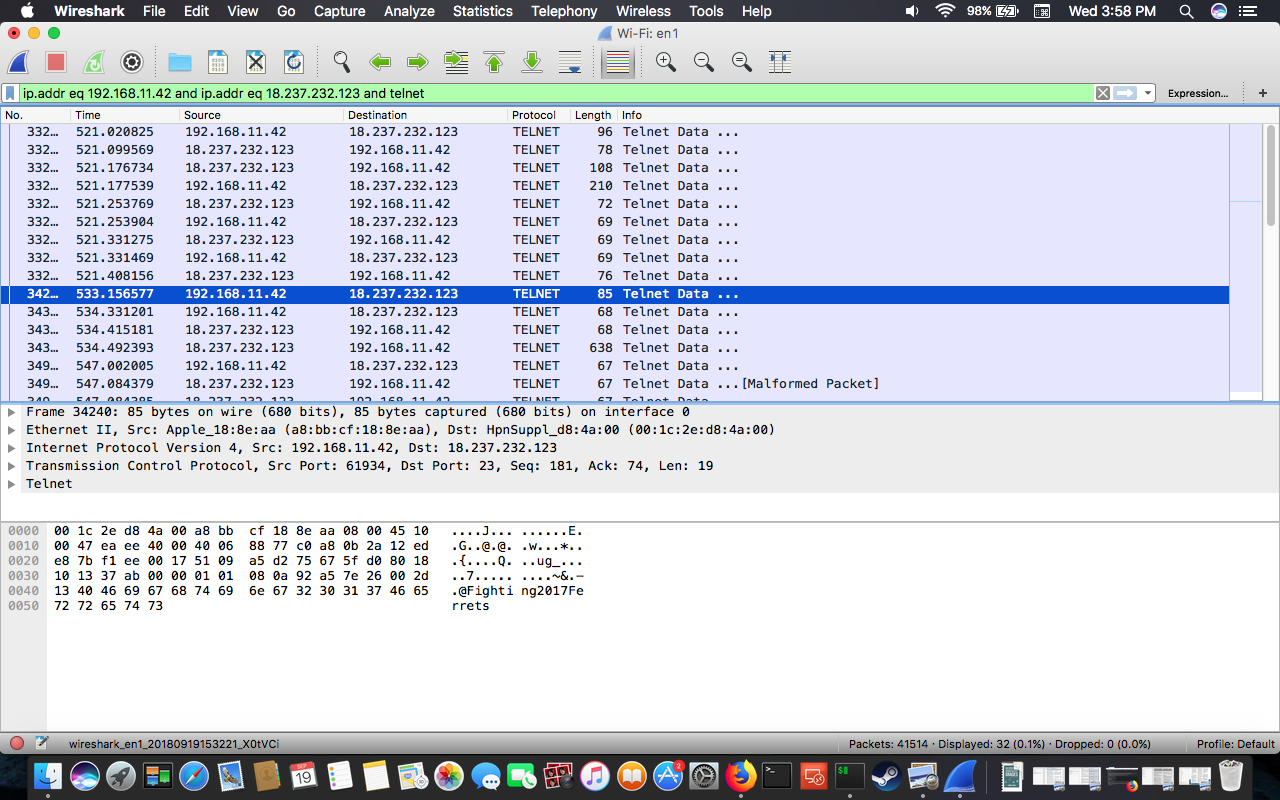
\includegraphics[width=\linewidth]{telnet3.png}
	\caption{Password response is Fighting2017Ferrets}
	\label{fig:telnet3}
\end{figure}

\section{Conclusion}

Encryption is an invaluable tool for keeping data secure, and should not be
ignored. In the modern era, there is no excuse to be using tools like Telnet,
or similarly unsecured protocols like HTTP when confidential information is
relevant. If you must use an unsecured protocol or program, you must assume
that someone other than your intended recipient is grabbing and perusing that
information. For some small website that has no user information or sensitive
data being transmitted, just site content, that may be fine, but for anything
with a login page, that's not okay.

\end{document}
